\chapter{PROBLEM 1}
\label{ch:p1}

\begin{center}\large\bfseries Yang Pulang Membawa Laptopnya\end{center}

\section{Identifikasi Masalah}

Pada M1, satu basis data menyimpan seluruh \texttt{HazardEvent}. Membagi data ke beberapa \emph{shard} menyebarkan pekerjaan penulisan, tetapi manfaatnya bergantung pada kunci partisi. Jika shard ditentukan dari wilayah, rentetan gempa di satu wilayah dapat menimbulkan \emph{hotspot} meskipun kapasitas total klaster masih tersedia. Setelah data dibagi, hilangnya satu node juga dapat menghilangkan satu bagian katalog. Karena itu, partisi perlu disertai replikasi dan mekanisme pemulihan ketika primary hilang \cite{kleppmann2017}.

Pembagian data memengaruhi pembacaan. Permintaan untuk 50 kejadian terbaru harus memeriksa setiap shard agar dapat menentukan urutan global. Bila satu shard lambat, menunggu seluruh hasil dapat membuat latensi permintaan mengikuti bagian yang paling lambat. Dampak ini terlihat pada \emph{tail latency}, yaitu latensi pada persentil tinggi \cite{dean2013}.

\section{Rancangan Solusi dan Mekanisme}

\subsection{Penempatan data dan pemulihan}

Aggregator menentukan shard dari pasangan \texttt{source} dan \texttt{source\_ref\_id}. Kedua nilai dipisahkan dengan byte NUL lalu di-hash dengan SHA-256. Delapan byte pertama dibaca sebagai bilangan tak bertanda. Sisanya terhadap 96 menentukan bucket, lalu sisa nomor bucket terhadap empat menentukan shard. Perubahan atribut kejadian, termasuk lokasi atau severity, tetap mengikuti identitas yang sama. Node baru atau node yang hilang hanya mengubah penempatan salinan fisik. Perubahan jumlah shard logis memerlukan migrasi pemetaan data.

Setiap shard mempunyai satu primary dan dua standby di tiga node berbeda. Kubernetes menegakkan penempatan tersebut melalui label dan aturan anti-affinity. PostgreSQL mengonfirmasi commit setelah WAL tersimpan di primary dan satu standby sinkron. Patroni mempromosikan standby yang memenuhi syarat bila primary hilang, sementara alamat Service untuk primary tetap sama. Dalam mode sinkron ketat, penulisan akan tertahan bila akhirnya tersisa satu salinan yang dapat menerima WAL \cite{patroni,postgres}. Trade-off ini menjaga data yang sudah diakui, dengan biaya latensi tambahan dan kemungkinan penulisan tertahan saat replikasi terganggu.

Volume bersifat lokal. Saat sebuah node diganti, node pengganti mengambil label penempatan yang kosong dan membangun ulang replika dari salinan yang masih tersedia. Setelah replikasi menyusul primary, \emph{switchover} terencana dapat memindahkan peran primary dan ikut memindahkan beban. Dengan cara ini, penambahan kapasitas fisik tetap memakai pemetaan data yang sudah berjalan.

\subsection{Pembacaan lintas shard dan konsistensi}

Permintaan daftar menggunakan pembacaan paralel ke primary setiap shard dan batas waktu pembacaan penyimpanan 200~ms. Aggregator menggabungkan kandidat dalam urutan \texttt{occurred\_at} menurun dan memakai urutan \texttt{hazard\_id} menaik bila waktu kejadian sama. Kursor membawa pasangan tersebut agar halaman berikutnya dapat dimulai dari batas yang sama pada semua shard. Bila suatu shard tidak menjawab sebelum tenggat, Aggregator menandai halaman sebagai parsial dan menahan kursor lanjutan. Pembaca dapat mengulang pemindaian setelah pulih tanpa melewatkan kejadian dari shard yang sebelumnya tak terjangkau.

Tabel~\ref{tab:p1-consistency} mencakup endpoint yang membaca data dan lokasi penyimpanan pada P1. Pembacaan normal melihat transaksi yang telah di-commit pada masing-masing primary. Karena setiap shard menjalankan transaksinya sendiri, hasil gabungan tidak menjanjikan satu snapshot global selama ada penulisan bersamaan. Jaminan tersebut berlaku pula pada pemindaian beberapa halaman Audit API. Untuk pemeriksaan checksum, data uji dijaga tetap agar kedua penghitungan dapat dibandingkan.

\begin{table}[htbp]
\centering\small
\caption{Jaminan pembacaan normal dan respons ketika satu node hilang. Baris Audit menggunakan awalan \texttt{/internal/audit}.}
\label{tab:p1-consistency}
\begin{tabularx}{\linewidth}{@{}lYY@{}}
\toprule
Endpoint & Kondisi normal & Saat pemulihan \\
\midrule
\texttt{/v1/hazards} & Daftar terurut lintas primary. & Daftar lengkap bila semua shard dapat dibaca, atau data yang tersedia dengan \texttt{partial}, daftar shard yang tak terjangkau, dan tanpa kursor berikutnya. \\
\texttt{/v1/hazards/\{id\}} & Mengembalikan kejadian aktif yang ditemukan. HTTP~404 bila ID tidak ada. & HTTP~200 bila ditemukan, atau HTTP~503 jika shard yang gagal masih mungkin menyimpan ID tersebut. \\
\texttt{/v1/analytics} & Agregat dari satu pernyataan SQL per primary. & Agregat dari shard yang dapat dibaca disertai \texttt{partial} dan informasi cakupan. \\
Audit \texttt{/events} & Daftar kejadian aktif, terurut menurut \texttt{ingested\_at} lalu \texttt{hazard\_id}. & Hasil parsial tanpa kursor berikutnya bila sebagian shard tak terjangkau. \\
Audit \texttt{/checksum} & SHA-256 atas ID referensi yang diurutkan per byte dan dipisah baris baru. & Hash dihitung dari ID yang terjangkau dan ditandai parsial. Hash ini hanya mewakili bagian tersebut. \\
Audit \texttt{/location} & Lokasi diperiksa pada setiap salinan PostgreSQL setelah shard diketahui. & Pencarian atau pemeriksaan salinan yang gagal ditandai parsial. HTTP~404 hanya bila semua primary dapat diperiksa dan ID tidak ditemukan. \\
Audit \texttt{/unprocessed} & Memindai catatan jurnal yang belum selesai pada shard asal setiap sumber. & Menandai hasil parsial bila jurnal yang dibutuhkan tak terjangkau. \\
\texttt{POST /field-reports} & HTTP~202 setelah commit di primary dan standby sinkron. Kunci dan payload sama memberi tanda terima sama, payload berbeda HTTP~409. & HTTP~503 dan \texttt{Retry-After} bila shard belum dapat mengonfirmasi. Tanda terima lama tetap ada di standby. \\
\texttt{GET /field-reports/\{id\}} & Mencari ID laporan di semua shard. & HTTP~404 hanya bila semua shard menjawab, selain itu HTTP~503. \\
\texttt{/failed-messages} & Daftar seperti Audit \texttt{/unprocessed}. Detail dan replay memakai jurnal di shard asal. & Daftar ditandai parsial. Detail dan replay HTTP~503 bila shard asal tak terjangkau. \\
\bottomrule
\end{tabularx}
\end{table}

\subsection{Agregasi untuk dasbor analitik}

Aggregator meminta setiap primary menghitung kejadian aktif dalam rentang $[\textit{from},\textit{to})$ menurut interval waktu, jenis bahaya, severity, dan \texttt{area\_name}. Ia menjumlahkan kelompok yang sepadan dari shard yang menjawab dalam 450~ms. Satu kejadian gempa dengan atribut \texttt{tsunami\_warnings} dapat masuk ke seri gempa dan seri tsunami. Pada total kejadian, distribusi severity, dan distribusi wilayah, kejadian tersebut tetap dihitung sekali.

Dasbor di \texttt{/analytics/} menggunakan \texttt{/v1/analytics} untuk menggambar seri waktu dengan pilihan rentang serta menyajikan distribusi severity dan wilayah. Jika sebagian shard gagal menjawab, dasbor tetap menyajikan hasil yang ada dengan peringatan data parsial dan jumlah shard yang berhasil dibaca. Perbandingan dengan Audit API memakai rentang \texttt{occurred\_at} dan aturan pengelompokan yang sama.

\section{Alasan Keputusan dan Trade-off}

Hash identitas menjaga pembaruan satu kejadian tetap berada pada shard yang sama sekaligus menyebarkan kejadian berbeda dari sumber atau wilayah yang sama. Tabel~\ref{tab:p1-partition} membandingkan dampaknya dengan dua pilihan lain.

\begin{table}[htbp]
\centering\small
\caption{Dampak pilihan kunci partisi terhadap sebaran penulisan.}
\label{tab:p1-partition}
\begin{tabularx}{\linewidth}{@{}lY@{}}
\toprule
Kunci & Dampak saat aktivitas terkonsentrasi \\
\midrule
Wilayah & Pembacaan satu wilayah dapat diarahkan ke satu shard, tetapi lonjakan di wilayah tersebut juga membebani satu primary. \\
Sumber & Riwayat per sumber mudah ditelusuri, tetapi seluruh lonjakan dari BMKG masuk ke shard yang sama. \\
Hash identitas & ID berbeda dari wilayah atau sumber yang sama dapat tersebar. Pembacaan lintas kejadian perlu menggabungkan hasil dari semua shard, sedangkan pembaruan berulang atas satu ID tetap menuju satu shard. \\
\bottomrule
\end{tabularx}
\end{table}

\section{Batasan yang Disadari}

Uji impor memakai CSV latihan. Checksum yang cocok mengonfirmasi kelengkapan 500 baris dalam skenario itu. Kehilangan disk dan penggantian worker sudah diuji dalam satu rangkaian pada klaster Azure tiga node, tetapi belum pada klaster Hetzner empat node. Setelah katalog dan checksum dari asisten tersedia, pengujian akhir untuk demonstrasi dapat memakai keduanya untuk memeriksa impor, lonjakan di satu wilayah, kehilangan disk, dan penggantian worker dalam satu rangkaian. Pada rangkaian itu, beban tiap node dan indikator parsial di dasbor juga perlu diukur.

Rancangan mengasumsikan satu kegagalan worker dalam satu waktu dengan control plane tetap tersedia. Hashing menyebarkan kejadian antarshard, sementara beban per node mengikuti penempatan primary. Pada Tabel~\ref{tab:p1-placement}, dua dari empat primary berada di \texttt{aat-dev}. \emph{Switchover} terencana dapat memindahkan beban bila pengukuran menunjukkan hotspot pada node tersebut.

\section{Bukti Penyelesaian}

\subsection{Penempatan, impor, dan urutan baca}

Tabel~\ref{tab:p1-placement} mencatat penempatan pada klaster Hetzner, 22 November 2026 pukul 13.38 WIB. Setiap shard memiliki tiga salinan di node berbeda, dengan primary tersebar pada tiga node.

\begin{table}[htbp]
\centering\small
\caption{Penempatan primary dan standby pada klaster Hetzner.}
\label{tab:p1-placement}
\begin{tabularx}{\linewidth}{@{}lYY@{}}
\toprule
Node & Primary & Standby \\
\midrule
\texttt{aat-dev} & \texttt{shard-1-0}, \texttt{shard-3-0} & \texttt{shard-2-2} \\
\texttt{aat-worker-1} & --- & \texttt{shard-0-1}, \texttt{shard-2-0}, \texttt{shard-3-2} \\
\texttt{aat-worker-2} & \texttt{shard-0-0} & \texttt{shard-1-1}, \texttt{shard-3-1} \\
\texttt{aat-worker-3} & \texttt{shard-2-1} & \texttt{shard-0-2}, \texttt{shard-1-2} \\
\bottomrule
\end{tabularx}
\end{table}

Pada klaster Hetzner, Audit API menemukan salinan satu \texttt{HazardEvent} pada tiga node. Inventaris klaster mencatat 12 salinan PostgreSQL dan tiga broker JetStream siap (Lampiran~\ref{app:evidence}).

Uji impor pada fixture PostgreSQL memakai 500 baris CSV sintetis dengan koordinat yang sama untuk memeriksa sebaran data dari satu wilayah. Impor dihentikan setelah 100 baris tercatat di jurnal, lalu dilanjutkan. Fungsi checksum Audit menghitung 500 ID dan mengembalikan \texttt{partial=false}. Nilainya sama dengan checksum dari ID pada CSV.

\terminalfigure{p1-import-checksum}{Perbandingan checksum CSV dan hasil pemeriksaan Audit dari uji impor yang tersimpan.}{fig:p1-import-checksum}

Jumlah kejadian pada \texttt{shard-0} hingga \texttt{shard-3} berturut-turut adalah 120, 120, 155, dan 105. Dengan demikian, shard terpadat menampung 31\% dari kejadian latihan meskipun seluruh masukan berasal dari satu lokasi. Angka ini mengukur distribusi penempatan baris. Pengukuran CPU dan laju tulis setiap node perlu dilakukan pada impor dan lonjakan katalog acuan.

Fixture PostgreSQL memeriksa kelanjutan impor tanpa duplikat. Uji dengan empat basis data memeriksa rute tulis, urutan lintas shard, dan kursor antarhalaman. Uji tambahan menahan satu shard melewati tenggat. Hasil yang terjangkau tetap dikembalikan dan halaman parsial tidak memajukan kursor. Pengujian urutan juga mencakup waktu dengan pecahan detik dan offset zona waktu yang berbeda.

\subsection{Kehilangan worker dan penambahan node}

Setelah satu VM worker lokal ditangguhkan dan dibangunkan kembali, Audit menemukan seluruh 6.040 ID awal di antara 6.068 ID. Selama uji, 140 permintaan dijawab tanpa galat HTTP, termasuk 21 respons parsial. Latensi tertinggi mencapai 873{,}5~ms. Klaster kembali memiliki 12 salinan setelah pulih.

Pada uji penambahan node di lingkungan lokal, worker tambahan menampung replika \texttt{shard-1}. Setelah menyusul primary, replika dipromosikan dan worker menangani pembacaan ke shard tersebut serta satu Aggregator. Peran primary dikembalikan setelah uji. Penggantian worker dengan disk kosong diuji pada klaster Azure.

\subsection{Kehilangan worker dan penggantian disk pada klaster Azure}

Uji ini memakai klaster Azure tiga node (Tabel~\ref{tab:topology-azure}) dan mengikuti cara pemeriksaan uji Hetzner: Audit API memindai seluruh \texttt{HazardEvent} sebelum dan sesudah gangguan, sementara probe membaca \texttt{/v1/hazards} melalui Auth dan Client API sepanjang uji. Sebelum gangguan, \texttt{aat-worker-1} memegang primary \texttt{shard-0} dan \texttt{shard-3}, standby \texttt{shard-1} dan \texttt{shard-2}, satu Aggregator, dan satu broker JetStream. VM tersebut dimatikan paksa tanpa proses shutdown. Sekitar 80~detik kemudian, objek node dan kelima volume lamanya (empat volume PostgreSQL dan satu volume JetStream) dihapus dari klaster. VM yang sama lalu dinyalakan kembali sehingga bergabung dengan disk kosong. Tabel~\ref{tab:p1-azure} merangkum hasilnya.

\begin{table}[htbp]
\centering\small
\caption{Kehilangan worker dan penggantian disk pada klaster Azure, 22 November 2026.}
\label{tab:p1-azure}
\begin{tabularx}{\linewidth}{@{}>{\raggedright\arraybackslash}p{0.33\linewidth}Y@{}}
\toprule
Pengamatan & Hasil \\
\midrule
Failover primary & \texttt{shard-0} pindah ke \texttt{aat-worker-2} dan \texttt{shard-3} pindah ke \texttt{aat-dev} tanpa intervensi. \\
Pembacaan 64~detik pertama & 201 dari 201 permintaan menerima HTTP~200, 40 di antaranya berpenanda \texttt{partial}. p95 204{,}8~ms dan latensi tertinggi 881{,}2~ms. \\
Pembacaan sejak kill hingga node pulih (324~detik) & 1.198 dari 1.198 permintaan menerima HTTP~200, termasuk 40 respons parsial. Tidak ada HTTP~500 maupun permintaan yang menggantung. \\
Kelengkapan data & Audit sebelum gangguan mencatat 3.062 kejadian (BMKG 49, PVMBG 48, Sensor Pantai 2.965). Sesudahnya tercatat 4.429 kejadian dan seluruh 3.062 ID awal masih ada, tanpa \path{source_ref_id} ganda. \\
Node bergabung dengan disk kosong & Empat replika PostgreSQL dan satu broker dibangun ulang pada volume baru. Ke-12 salinan dan JetStream kembali siap 172~detik setelah node bergabung. \\
Node ikut menanggung beban & \emph{Switchover} Patroni memindahkan primary \texttt{shard-0} ke \texttt{aat-worker-1}, sehingga node itu kembali menanggung beban tulis. \\
Redundansi pulih & \texttt{check-cluster.py} kembali lolos: setiap shard memiliki standby sinkron di node lain. \\
\bottomrule
\end{tabularx}
\end{table}

Uji ini belum memakai checksum resmi dari asisten, sehingga kelengkapan diperiksa dari himpunan ID Audit sebelum dan sesudah gangguan. Log dan skripnya tersedia di \path{docs/report-m2/evidence/azure}.

\subsection{Kesesuaian agregat dengan Audit API}

Pada klaster lokal, dasbor dan Audit API sama-sama menghitung 120 kejadian pesisir untuk 12 November 2026 pukul 00.00 hingga sebelum 00.30 UTC (Gambar~\ref{fig:p1-dashboard}). Fixture dengan enam kejadian juga menghasilkan angka yang sama dari kedua API pada lima seri bahaya. Satu gempa muncul pada seri gempa dan tsunami, tetapi hanya dihitung sekali dalam total.

\begin{figure}[H]
\centering
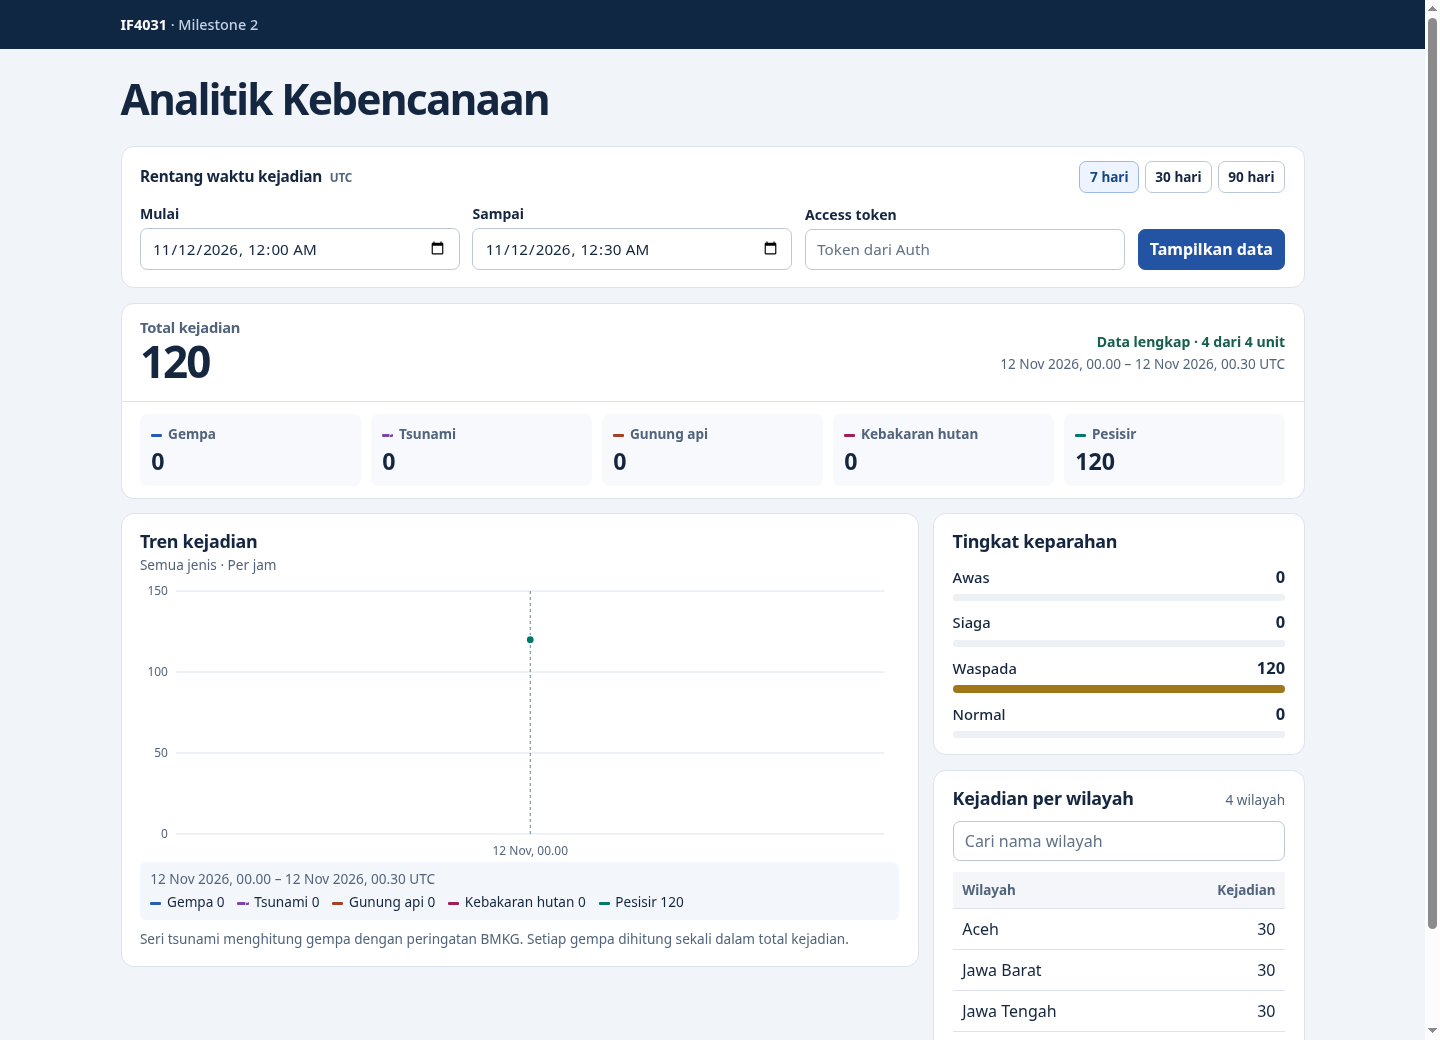
\includegraphics[width=0.90\linewidth]{figures/analytics.png}
\caption{Dasbor Analitik pada klaster lokal dengan data Sensor Pantai.}
\label{fig:p1-dashboard}
\end{figure}

\section{Jawaban atas Butir ``Di laporan''}

\begin{table}[H]
\centering\small
\begin{tabularx}{\linewidth}{@{}>{\raggedright\arraybackslash}p{1.6cm}>{\raggedright\arraybackslash}p{3.4cm}>{\raggedright\arraybackslash}p{3.3cm}Y@{}}
\toprule
Kriteria & Persoalan & Istilah literatur & Mekanisme kelompok \\
\midrule
K1, K2 & Data tidak muat di satu tempat dan beban terpusat pada wilayah ramai & \emph{Partitioning}, \emph{skew}, \emph{hotspot} & Hash SHA-256 atas \texttt{source} dan \texttt{source\_ref\_id} ke 96 bucket dan 4 shard \\
K3, K7 & Daftar dan agregat harus menggabungkan semua shard & \emph{Scatter-gather}, \emph{tail latency} & Pembacaan paralel dengan tenggat 200 dan 450~ms serta penanda \texttt{partial} \\
K4, K6 & Data hilang bersama node & \emph{Replication}, \emph{failover} & Tiga salinan per shard, standby sinkron, promosi Patroni \\
K5 & Node baru harus ikut menanggung beban & \emph{Rebalancing} & Replika dibangun ulang pada node baru, lalu \emph{switchover} \\
\bottomrule
\end{tabularx}
\caption{Ringkasan persoalan dan mekanisme P1.}
\label{tab:p1-ringkas}
\end{table}

\noindent\begin{minipage}{\linewidth}
\begin{lstlisting}[caption={Penentuan shard dari identitas kejadian.},label={code:p1-partition}]
// services/aggregator/internal/partition/partition.go
func Unit(source contracts.Source, refID string) (string, error) {
	if !source.Valid() || refID == "" {
		return "", errors.New("valid source and reference ID required")
	}
	sum := sha256.Sum256([]byte(string(source) + "\x00" + refID))
	bucket := binary.BigEndian.Uint64(sum[:8]) % BucketCount
	return fmt.Sprintf("shard-%d", bucket%UnitCount), nil
}
\end{lstlisting}
\end{minipage}


\begin{enumerate}
\item \textbf{Persoalan dan namanya dalam literatur.} Problem ini memuat empat persoalan. Pertama, \emph{partitioning} atau \emph{sharding}: satu basis data tidak lagi menampung seluruh kejadian, sehingga data dibagi ke beberapa unit. Kedua, \emph{skew} atau \emph{hotspot}: kunci partisi yang mengikuti wilayah atau sumber memusatkan beban pada satu unit ketika gempa terkonsentrasi di satu jalur. Ketiga, \emph{replication} dan \emph{failover}: data yang hanya disimpan di satu node hilang bersama node tersebut, sehingga setiap unit memerlukan salinan dan pemilihan primary baru. Keempat, \emph{rebalancing}: node baru harus ikut menanggung data tanpa menghentikan layanan \cite{kleppmann2017}. Pembacaan lintas shard juga menghadapi persoalan \emph{scatter-gather} dan \emph{tail latency}, karena hasil gabungan menunggu shard yang paling lambat \cite{dean2013}.

\item \textbf{Mekanisme penempatan data.} Aggregator menghitung SHA-256 atas pasangan \texttt{source} dan \texttt{source\_ref\_id}, membaca delapan byte pertama sebagai bilangan, lalu memetakannya ke 96 bucket dan empat shard logis. Pemetaan ini tidak bergantung pada node, sehingga satu kejadian selalu menuju shard yang sama. Ketika node datang atau pergi, yang berubah hanya penempatan salinan fisik. Label node dan aturan anti-affinity menentukan node yang berhak menampung salinan. Saat primary hilang, Patroni mempromosikan standby sinkron. Node pengganti mengambil label yang kosong dan membangun ulang replika dari salinan yang tersisa. Setelah replika menyusul, \emph{switchover} terencana dapat memindahkan peran primary ke node tersebut. Perubahan jumlah shard logis tetap memerlukan migrasi pemetaan.

\item \textbf{Perbandingan pendekatan alternatif.} Tabel~\ref{tab:p1-partition} membandingkan tiga kunci partisi. Partisi menurut wilayah memusatkan lonjakan gempa pada satu primary. Partisi menurut sumber menempatkan seluruh data BMKG pada satu shard, sehingga ketidakmerataan antarsumber langsung menjadi ketidakmerataan beban. Hash identitas menyebarkan kejadian dari wilayah yang sama. Pada uji impor 500 baris dengan koordinat yang sama, shard terpadat menampung 31\% kejadian. Konsekuensinya, pembacaan daftar harus menggabungkan hasil dari semua shard, dan beban per node masih mengikuti letak primary, yang dapat diseimbangkan dengan \emph{switchover}.

\item \textbf{Jaminan konsistensi per endpoint.} Tabel~\ref{tab:p1-consistency} merinci jaminan setiap endpoint. Pada kondisi normal, pembacaan melihat transaksi yang sudah di-commit pada primary masing-masing shard, tetapi hasil gabungan tidak membentuk satu snapshot global karena setiap shard bertransaksi sendiri. Penulisan baru diakui setelah WAL tersimpan di primary dan satu standby sinkron, sehingga data yang sudah diakui tidak hilang saat satu node hilang. Selama pemulihan, endpoint daftar dan agregat mengembalikan data yang tersedia dengan penanda \texttt{partial} dan daftar unit yang tidak terjangkau. Endpoint yang mencari satu ID mengembalikan HTTP~503 bila shard yang mungkin menyimpan ID tersebut belum terjangkau, agar ketiadaan data tidak disimpulkan secara keliru. Pilihan ini mengutamakan kebenaran jawaban di atas kelengkapan selama partisi jaringan atau failover berlangsung.

\item \textbf{Agregasi dasbor analitik.} Aggregator meminta setiap primary menjalankan satu pernyataan SQL yang mengelompokkan kejadian aktif dalam rentang $[\textit{from},\textit{to})$ menurut interval waktu, jenis bahaya, severity, dan \texttt{area\_name}. Hasil dari shard yang menjawab dalam 450~ms dijumlahkan per kelompok. Kejadian gempa yang memuat peringatan tsunami masuk ke seri gempa dan tsunami, tetapi dihitung sekali pada total, distribusi severity, dan distribusi wilayah. Bila ada shard yang tidak menjawab, respons membawa \texttt{partial} beserta jumlah shard yang berhasil dibaca, dan dasbor menampilkan peringatan data parsial bersama angka tersebut. Angka dasbor dibandingkan dengan Audit API memakai rentang \texttt{occurred\_at} dan aturan pengelompokan yang sama.
\end{enumerate}
